\documentclass[conference]{IEEEtran}
\usepackage{cite}
\usepackage{amsmath,amssymb,amsfonts}
\usepackage{algorithmic}
\usepackage{graphicx}
\usepackage{textcomp}
\usepackage{xcolor}
\def\BibTeX{{\rm B\kern-.05em{\sc i\kern-.025em b}\kern-.08em
    T\kern-.1667em\lower.7ex\hbox{E}\kern-.125emX}}
\begin{document}

\title{COS 711 Assignment 2\\
{\footnotesize Supervised Neural Network Training}
}

\author{\IEEEauthorblockN{Jeffrey Russell (u16010648)}
\IEEEauthorblockA{\textit{EBIT} \\
\textit{University of Pretoria}\\
Pretoria, South Africa \\
u16010648@tuks.co.za}
}

\maketitle

\begin{abstract}
In this project we were instructed to implement a neural network with
automatic architecture selection and curriculum learning on two wine quality
datasets. There were numerous hurdles to overcome such as the nature of the data
and the imbalance of the classes given. The final results were promising with 
an accuracy of approximately 70\% finally being achieved on the red wine.
\end{abstract}

\begin{IEEEkeywords}
neural networks, curriculum learning
\end{IEEEkeywords}

\section{Introduction}
In this project we were given a dataset containing a number of wine traits
(ph, density, etc.) and the subjective quality assigned by a human. My goal was
to create a neural network with certain added extras that would be able to predict
the quality of the wine given the set of wine traits of any particular wine. The
majority of the work fell into four different pieces of this program: preprocessing,
manual parameter tuning, auto architecture selection, and a curriculum learning algorithm.

The results were promising, achieving good accuracy on the two datasets, but
they did seem a bit underwhelming considering the difficulty to produce them.

\section{Background}
The preprocessing of the data was fairly simple because Python has so many built-in
packages for doing data manipulation and processing. The pre processing involved some
statistical analysis and the PCA algorithm to remove useless properties of the wine, 
and reduce the dimensionality of the problem for the NN.
\\\\
After the preprocessing, the next step was to create the neural network itself.
I used Tensorflow for the neural network itself with categorical cross entropy
as the loss function (this isn't the full story on the loss function, more on that later).
The preprocessing step took care of the test/generalization/global split. The 
parameter tuning that I did to come up with an optimal neural network architecture
and training strategy was fairly emperical, trying different values and seeing
what worked and what didn't.
\\\\
Insert auto architecture selection piece here
\\\\
The curriculum learning part of the project ended up being fairly simple, though
it was very long running. I created a GA which decides on the order
of the samples shown to the neural network in a number of batches.
It progressively shows the NN more and more samples until in the final batch
all of the samples are present.


\section{Experimental set-up}
I've split the experimental set-up into the four different parts of the project.

\subsection{Preprocessing}
I loaded the data through pandas from the csv files and then used scipy and numpy to split up the data and do the preprocessing.
The data was first sent through a z-score estimation function (provided by scipy.stats) which assumes a normal distribution of each input variable and then gives each value a z-score based on the mean and standard deviation within the input variable.
\\\\
The assumption of a normal distribution seemed justifiable since since most of the qualities are based on biological processes within the fermentation of wine that should present normal distribution curves when examined across a sufficiently large sample size. A couple of the input variables were fairly skewed to one side or the other, but the removal of outliers and increase in variation that the z-score introduced would seem to outweigh the possible problems with this approach.
\\\\
I then removed all rows in the data which had a column that was more than three standard deviations away from the mean. This dealt with outliers nicely and made the rest of the process much simpler. I also reduced the range of the values to between 0 and 1. In order to deal with class imbalance I decided to use a cost-sensitive loss function based on how many samples there were of that kind, the exact equation for the loss is described in the neural network architecture section.
\\\\
The next step for the preprocessing was to apply a PCA to the dataset in order to throw away the least useful input variables. I decided to throw away two of the input variables since that seemed to work well. That reduced the dimensionality of the input from 11 down to 9.
\\\\
The final step was to split the data into training/testing and global generalization. The percentages I decided on was 70\% for training and then 15\% each for testing and global generalization. This split was decided on because it seemed to give good results without cutting down too much on the testing size. This was all done with the red wine dataset in mind which is a bit smaller so that influenced the decision a bit. Because all the processing steps happened before the split between test and training data, there might have been some latent information based on the preprocessing that might have slightly increased the accuracy, but I don't think that it would be enough to warrant a different approach.

\subsection{Neural network}
The neural network was created in Tensorflow with Keras as the backend. I did a lot of experimentation trying to work out which particular parameters ended up creating the best and quickest convergence. Not everything that I did I have graphs for, but the most important stuff I do. The loss function that I used was categorical cross entropy (ish, I'll discuss the loss function below since it has some interesting quirks and rationale behind it). I decided on this because it seems to be the standard for measuring loss on categorical data across the sources that I reviewed.
\\\\
The input layer uses the tanh activation function. The hidden layers ended up just being a set of five layers with 9 neurons each all with activation function tanh. The output layer has 10 neurons with sigmoid activation. The input activation function is tanh because as soon as I tried any other activation function I immediately got a NaN loss in tensorflow. It seems to be because of the range of the output combined with the loss function which is categorical crossentropy which has issues with predictions of exactly zero since it has to do the log of that which causes undefined math operations. The hidden layers are all tanh since that had the best accuracy at a low number of epochs and a comparable accuracy further on. See fig \ref{fig:activation_type_loss} and \ref{fig:activation_type_accuracy} which compared relu, tanh, sigmoid and linear over 500 epochs running each model 100 times. Interestingly sigmoid is absolutely terrible up until about generation 300, and I have no idea why this might be.
\begin{figure}
  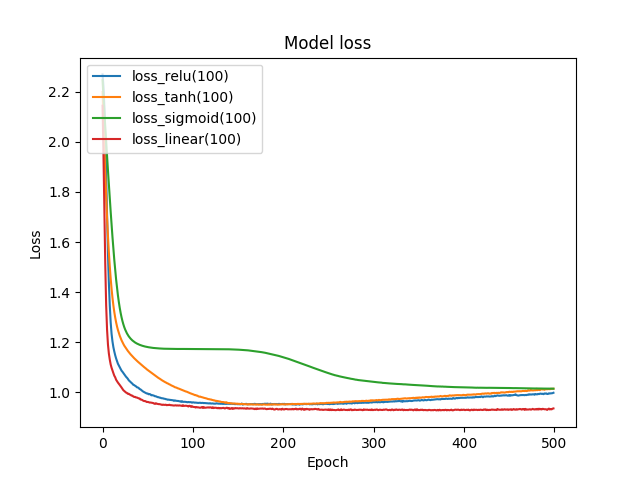
\includegraphics[width=\linewidth]{figs/different_activation_types_loss.png}
  \caption{Epoch number vs loss for four different activation functions}
  \label{fig:activation_type_loss}
\end{figure}
\begin{figure}
  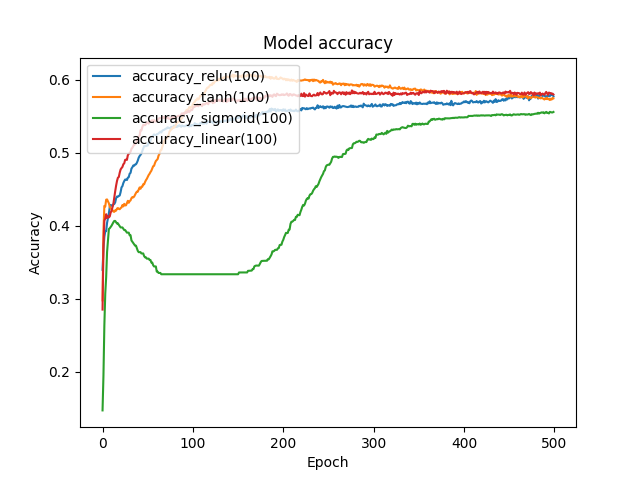
\includegraphics[width=\linewidth]{figs/different_activation_types_accuracy.png}
  \caption{Epoch number vs model accuracy for four different activation functions}
  \label{fig:activation_type_accuracy}
\end{figure}
\\\\
Because of the data shown in figure \ref{fig:activation_type_loss} and \ref{fig:activation_type_accuracy} I decided to have a minimum of 200 epochs with an ending function. This function takes a look at the last five epochs. For each epoch it considers the loss function result on the test data and compares that to the result for the current epoch. If 3 out of the most recent five have lower losses than the current epoch then the training is aborted. This exact function seems to strike an excellent balance between stopping too early based on a false positive and stopping too late because it didn't see the trend. As soon as the test loss starts increasing consistently it stops the training. This tends to happen right around the 200 epoch mark hence my use of 200 as my minimum epoch number.
\\\\
The batch size of 64 was decided on after trying to optimize for speed of convergence and final loss. As can be seen from figures \ref{fig:batch_size_loss}, \ref{fig:batch_size_accuracy} and \ref{fig:batch_size_time} the optimimum for time seems to be between 32, 64 and 128. I had originally picked 64 before doing the comparison and the loss and accuracy seem to support it as being very comparable. The fact that there's a bump in the middle for batch size of 64 doesn't really make sense and I'm pretty sure it's just a fluke with my setup so I'm assuming that 64 is actually the fastest running batch size.
\begin{figure}
  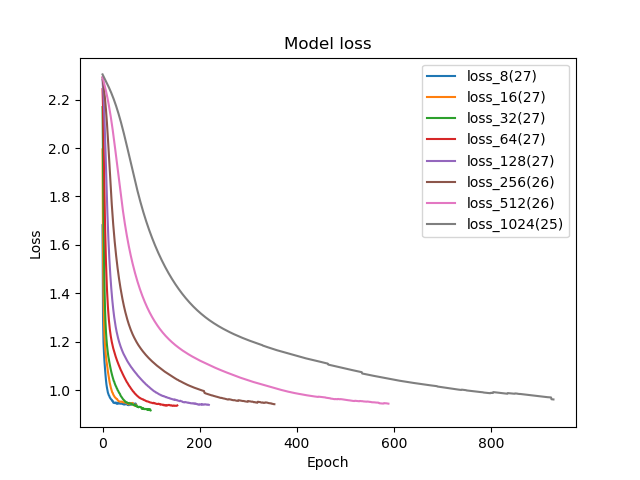
\includegraphics[width=\linewidth]{figs/batch_size_loss.png}
  \caption{Epoch number vs loss for eight different batch sizes}
  \label{fig:batch_size_loss}
\end{figure}
\begin{figure}
  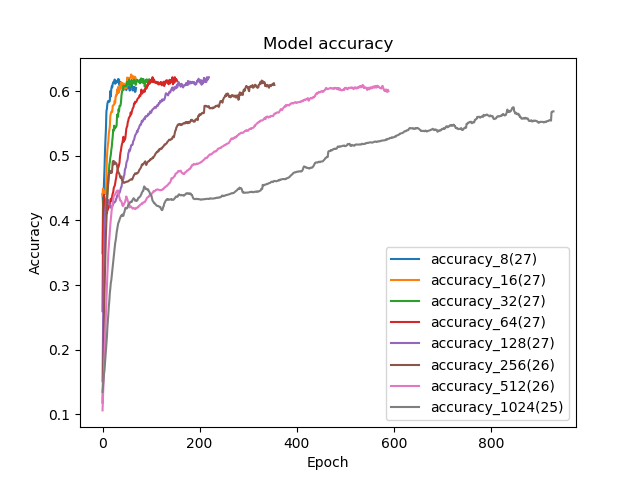
\includegraphics[width=\linewidth]{figs/batch_size_accuracy.png}
  \caption{Epoch number vs accuracy for eight different batch sizes}
  \label{fig:batch_size_accuracy}
\end{figure}
\begin{figure}
  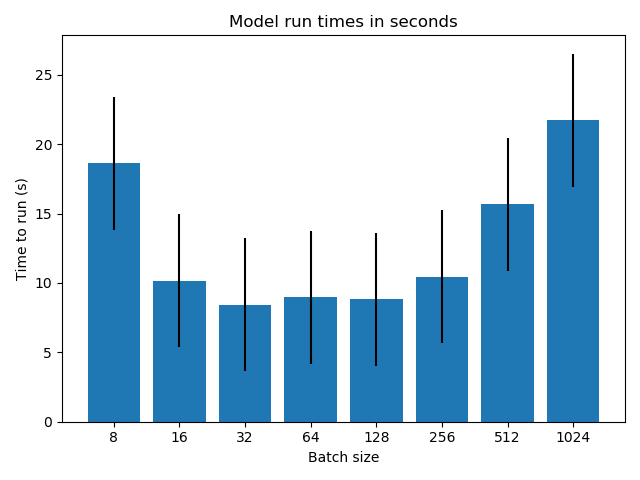
\includegraphics[width=\linewidth]{figs/batch_size_times.png}
  \caption{Length of time in seconds for eight different batch sizes to run}
  \label{fig:batch_size_time}
\end{figure}


\subsection{Automatic architecture selection}
I attempted an automatic architecture selection algorithm but was unable to get it working in time for the submission.
It involved a genetic algorithm similar to the one I implemented for the curriculum learning piece which was allowed to change the values of the architecture either in number of neurons or type of activation function. On a very small chance it also either added or subtracted a layer.

\subsection{Curriculum learning}
The curriculum learning approach was to create an ordering of the samples and then showing the NN the first set and then expanding that set of samples over time. The best ordering of the samples was created using a very basic GA with only mutation enabled. The genes of each member of the population was a list of numbers which correspond to samples in the data. The data coming in is always in the same order, so a particular sample of the data can be referred to simply by its row number. This is how the individuals in the population determine the ordering of the samples being shown to the neural network.
\\\\
The method of showing samples to the NN works in batches. I decided on five batches because it neatly divided the dataset into sets of about 200 which was the optimal number of epochs discovered in the previous section (These don't really have any real relation that I could think of). In the case of five batches the NN is shown the first fifth of the training set (according to the GA output ordering) for 40 epochs (200/5). In the next 40 epochs it is then shown the first two fifths of the training set, until for the final 40 epochs the NN is shown the entire data set to train on.
This worked quite well, and it gives an easily obtainable difficulty for samples depending on where they tend to end up in the order that the GA produces. I stumbled upon this way of creating the curriculum after reading through a number of different methodologies and realizing that this particular method fit well with the type of data and the other pieces of the puzzle that make up the classifier. 

\section{Research results}
The best final accuracy achieved was 68\%+-3\% on the red wine data set after using the curriculum learning to optimize the ordering. Without the curriculum learning the final results seemed to be about 62\%+-3\%. This difference seems to make sense as the curriculum learning is optimizing for accuracy, hence even if it isn't doing anything even vaguely related to actual curriculum learning because it is a GA running the neural network over and over again trying to find a better outcome, it will find that better outcome in whatever way possible.

\section{Conclusion}
In conclusion, the final accuracy seemed quite good and the project as a whole taught me a great deal about curriculum learning and automatic architecture selection.

\bibliographystyle{IEEEtran}
\bibliography{IEEEabrv,u16010648assignment2}

\vspace{12pt}

\end{document}
